\chapter{Sample Selections and Systematics}
\label{chap:SelsAndSysts}

\section{Systematic Uncertainties}
\label{sec:SelsAndSysts_Systs}

The systematics for this uncertainty are split into the groups, or blocks, depending on their purpose. They consist of flux uncertainties, neutrino-matter interaction systematics and detector efficiencies. There are also uncertainties on the oscillation parameters which this analysis will not be sensitive to, \delmsqsol and \sinsqsol. As described in \autoref{chap:MarkovChainMonteCarlo}, each model parameter used within this analysis requires a prior uncertainty. This is provided via separate covariance matrices for each block. The covariance matrices can include prior correlations between parameters within a single block, but the separate treatment means prior uncertainties can not be included for parameters in different groups. Alternatively, some parameters have no reasonably motivated uncertanities. These parameters are assigned flat priors which do not change the likelihood penalty. The flux, neutrino interaction and detector modelling has already been discussed in \autoref{sec:Simulations_Simulation}. The uncertainties invoked within these models are described below.

\subsection{Beam Flux}
\label{sec:SelsAndSysts_Systs_BeamFlux}

The neutrino beam flux systematics are based upon our uncertainty in the modelling of the components of the beam. This includes: the hadron production model and their re-interactions, the shape, intensity and alignment of the beam with respect to the target, and the uniformity of the magnetic field produced by the horn, alongside other effects. The uncertainty, as a function of neutrino energy, is illustrated in \autoref{fig:SelsAndSysts_BeamFluxSysts} which includes the total uncertainty as well as the individual components. The uncertainty for events below, and much higher than, the peak neutrino energy is dominated by hadron production and re-interaction systematics. The beam profile and alignment of the proton beam dominates the systematic uncertainty for events with \quickmath{E_{\nu} \sim 1\text{GeV}}. 

\begin{figure}[h]
  \begin{subfigure}[t]{\textwidth}
    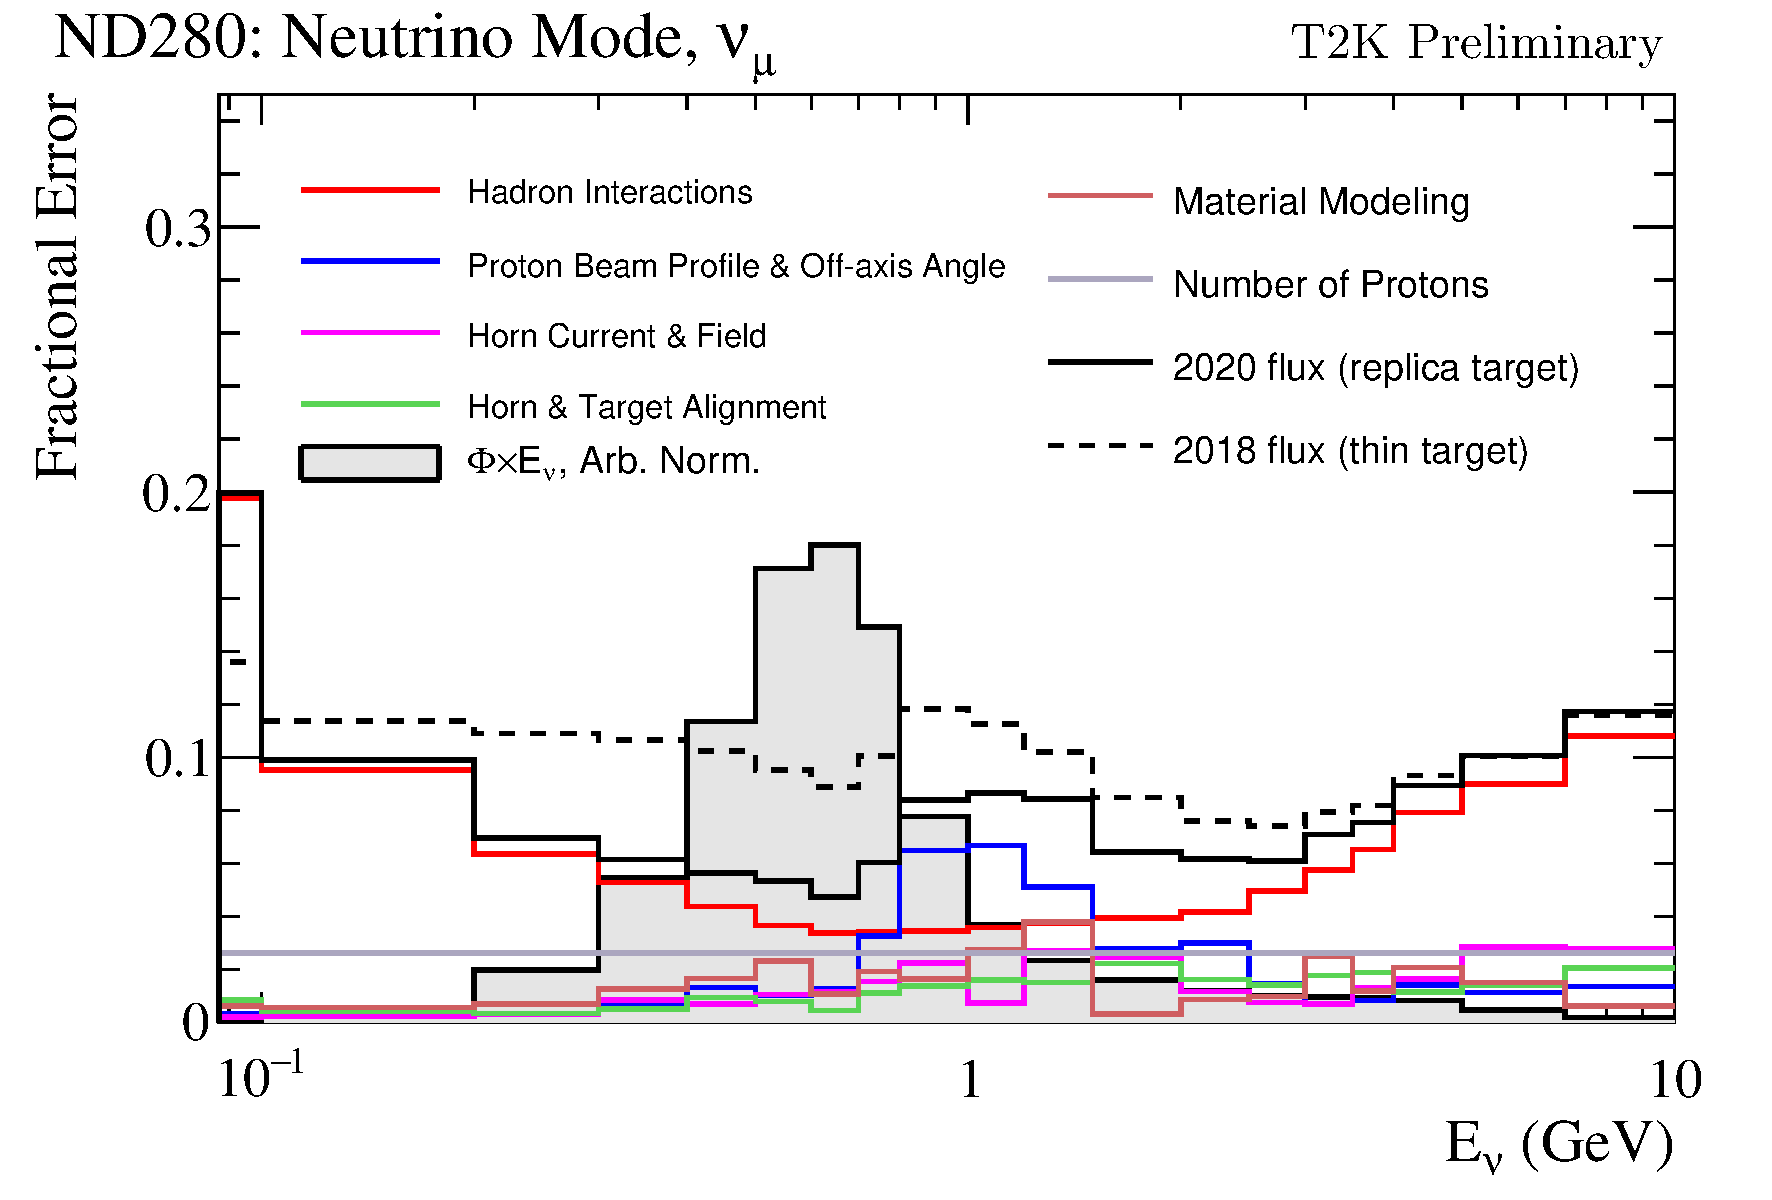
\includegraphics[width=\textwidth, trim={0mm 0mm 0mm 0mm}, clip,page=1]{Figures/Selections/flux_uncertainty_covariance_plots_addcorrnd_compwv3_flux_error_t2k_nd5_fhc_numu.pdf}
  \end{subfigure}
  %\begin{subfigure}[t]{\textwidth}
  %  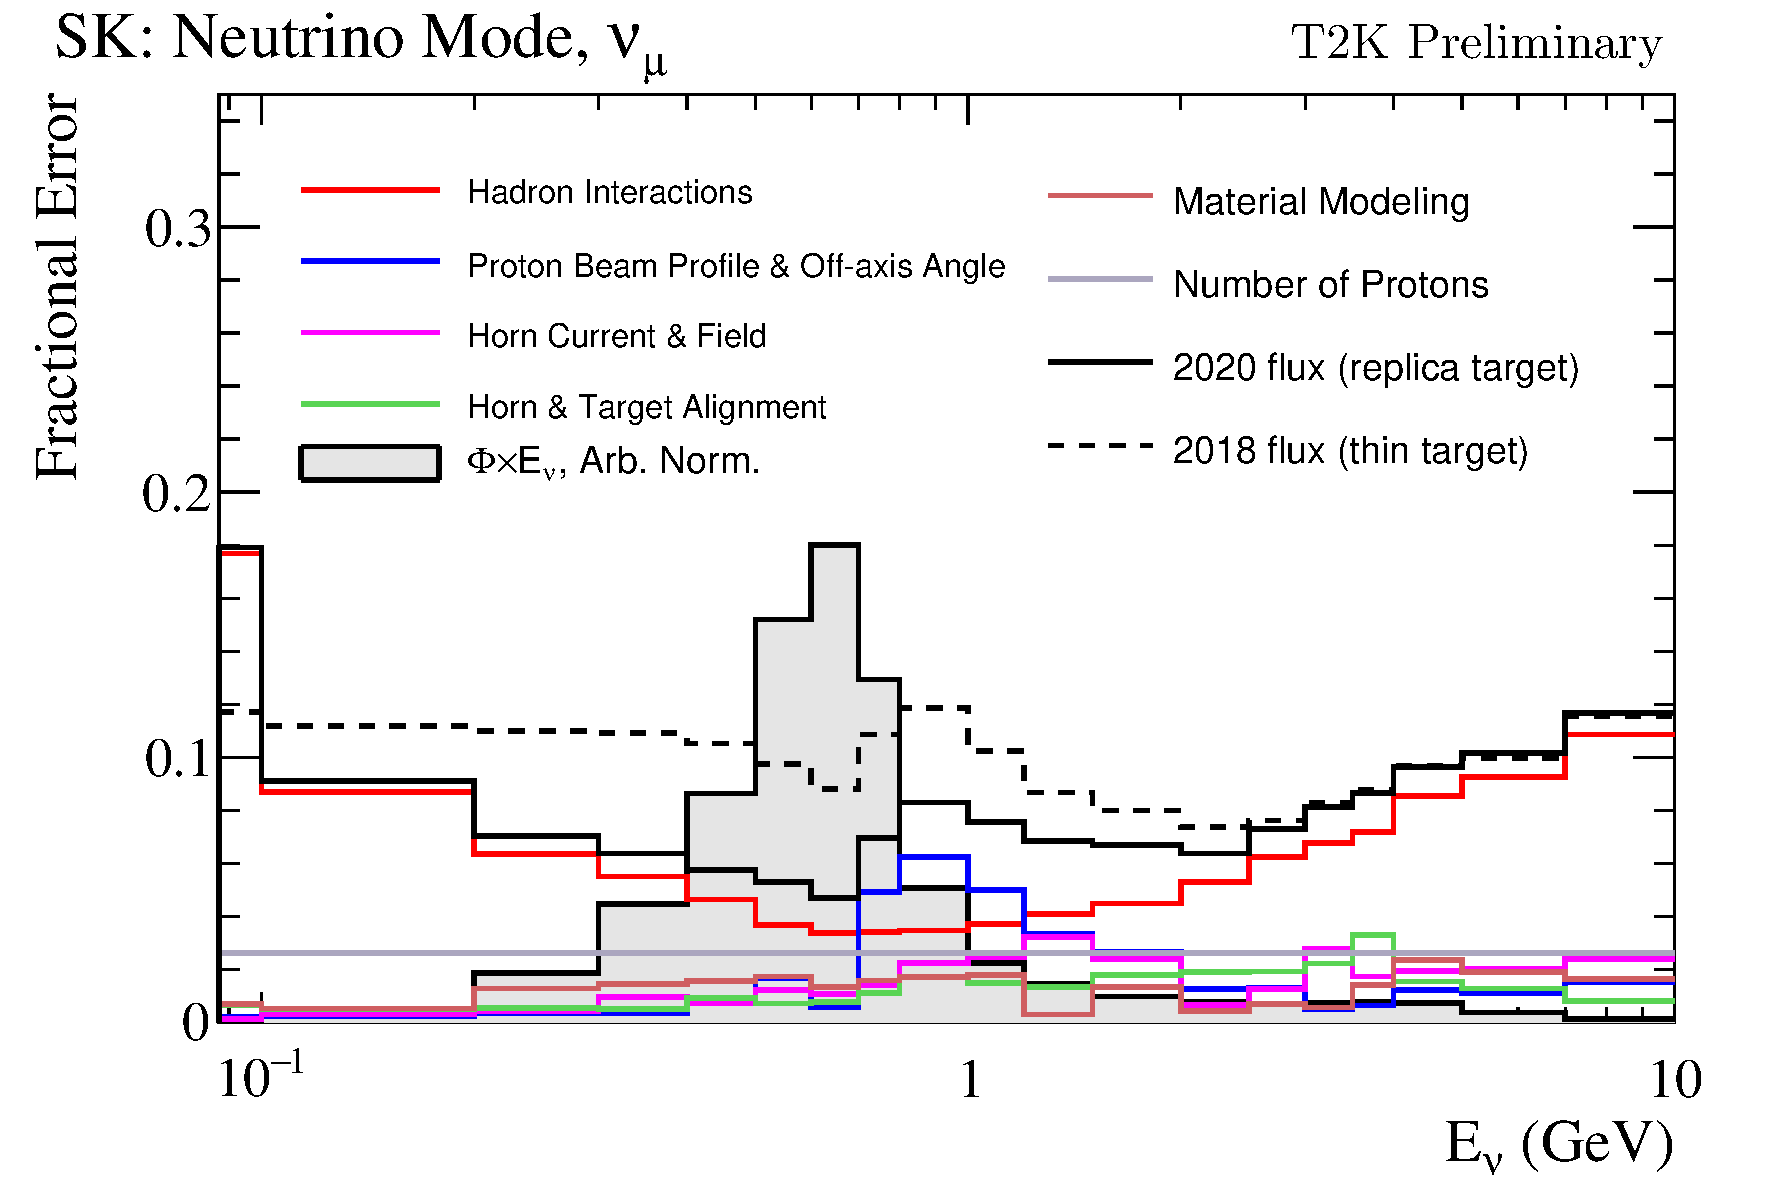
\includegraphics[width=\textwidth, trim={0mm 0mm 0mm 0mm}, clip,page=1]{Figures/Selections/flux_uncertainty_covariance_plots_addcorrnd_compwv3_flux_error_t2k_sk_fhc_numu.pdf}
  %\end{subfigure}
  \caption{The total uncertainty evaluated on the near detector \quickmath{\nu_{\mu}} flux prediction constrained by the replica-target data, illustrated as a function of neutrino energy. The solid(dashed) line indicates the uncertainty used within this analysis(the T2K 2018 analysis). The solid histogram indicates the neutrino flux as a function of energy. Figure taken from \cite{t2k_tn_354}.}
  \label{fig:SelsAndSysts_BeamFluxSysts}
\end{figure}

The beam flux uncertainties are described by one hundred parameters. They are split between both ND280 and SK detectors and binned by neutrino flavour: \quickmath{\nu_{\mu}}, \quickmath{\bar{\nu}_{\mu}}, \quickmath{\nu_{e}} and \quickmath{\bar{\nu}_{e}}. The response is then broken down as a function of neutrino energy. The bin density in the neutrino energy is the same for the FHC-\quickmath{\nu_{\mu}} and RHC-\quickmath{\bar{\nu}_{\mu}}, and narrows for neutrino energies close to the oscillation maxima of \quickmath{E_{\nu} = 0.6\text{GeV}}. This binning is specified in \autoref{tab:SelsAndSysts_BeamFluxBinEdges}. All of these systematic uncertanties are applied as normalisation parameters with Gaussian priors centered at \quickmath{1.0} and error specified from a covariance matrix provided by the T2K beam group.

\begin{table}[ht!]
    \centering
    \begin{tabular}{c|c|c}
      \hline
      Neutrino Flavour & Sign & Neutrino Energy Bin Edges (GeV) \\
      \hline
      \quickmath{\mu} & Right & \quickmath{0.,0.4,0.5,0.6,0.7,1.,1.5,2.5,3.5,5.,7.,30.} \\
      \quickmath{\mu} & Wrong & \quickmath{0.,0.7,1.,1.5,2.5,30.} \\
      \quickmath{e} & Right & \quickmath{0.,0.5,0.7,0.8,1.5,2.5,4.,30.} \\
      \quickmath{e} & Wrong & \quickmath{0.,2.5,30.} \\
      \hline
      \hline
    \end{tabular}
    \caption{The neutrino energy binning for the different neutrino flavours. ``Right'' sign indicates neutrinos in the FHC beam and antineutrinos in the RHC beam mode. ``Wrong'' sign indicates antineutrinos in the FHC beam and neutrinos in the RHC beam mode. The binning of the detector response is identical for the FHC and RHC modes as well as at ND280 and SK.}
    \label{tab:SelsAndSysts_BeamFluxBinEdges}
\end{table}

\subsection{Atmospheric Flux}
\label{sec:SelsAndSysts_Systs_AtmFlux}
The atmospheric neutrnio flux is modelled by the HKKM model, however 16 systematic uncertainties are applied to control the normalisation of each neutrino flavour, energy and direction. All of the parameters are given Gaussian priors centered at \quickmath{0} and width \quickmath{1.}. They are summarised below:

\begin{itemize}
\item \textbf{Absolute Normalisation}: The overall normalisation of each neutrino flavour is controlled by two indpendent systematic uncertainties, for \quickmath{E_{\nu} < 1\text{GeV}} and \quickmath{E_{\nu} > 1\text{GeV}}, respectively. This is driven mostly by hadronic interaction uncertainties for the production of pions and kaons \cite{Honda_2007}. The strength of the response is dependent upon the neutrino energy.
\item \textbf{Relative Normalisation}: Uncertainties on the ratio of \quickmath{(\nu_{\mu} + \bar{\nu}_{\mu})/(\nu_{e} + \bar{\nu}_{e})} are controlled by the difference between the HKKM model \cite{Honda_2007}, FLUKA \cite{etde_20239111} and Bartol models \cite{Barr_2004}. Three independent parameters are applied in the energy ranges: \quickmath{E_{\nu} < 1\text{GeV}}, \quickmath{1\text{GeV} < E_{\nu} < 10 \text{GeV}}, and \quickmath{E_{\nu} > 10\text{GeV}}.
\item \textbf{\quickmath{\nu}/\quickmath{\bar{\nu}} Normalisation}: The uncertainties in the \quickmath{\pi^{+}/\pi^{-}} (and kaon equivalent) produce uncertainties in the flux of \quickmath{\nu/\bar{\nu}}. The response is applied in the same way as the relative normalisation parameters.
\item \textbf{Up/Down and Vertical/Horizontal Ratio}: Similar to the above two systematics, the difference between the HKKM, FLUKA and Bartol model predictions, as a function of \quickmath{\cos(\theta_{Z})}, is used to control the normalisation of events as a function of zenith angle.
\item{\textbf{\quickmath{K/\pi} Ratio}}: Higher energy neutrinos (\quickmath{E_{\nu} < 10\text{GeV}}) become dependent upon kaon decay as the dominant source of neutrinos. Measurements of the ratio of \quickmath{K/\pi} \cite{Ambrosini1998-er} are used to control the systematic uncertainty of the expected ratio of pion and kaon production.
\item \textbf{Solar Activity}: As the 11-year solar cycle can affect the Earth's magnetic field, the flux of primary cosmic rays is modulated across the same period. The uncertainity is calculated by taking a \quickmath{\pm 1} year variation, equating to a \quickmath{10\%} uncertainty for the SK-IV period.
\item \textbf{Atmospheric Density}: The height of the interaction of the primary cosmic rays is dependent upon the atmospheric density. The HKKM assumes the US standard 1976 \cite{USStandardAtm} profile. This systematic controls the uncertainty in that model.
\end{itemize}

Updates to the HKKM and Bartol models are underway to use a similar tuning technique to that used in the beam flux predictions. After those updates, it may be possible to include correlations in the hadron production uncertanty systematics for beam and atmospheric flux predictions.

\subsection{Neutrino Interaction}
\label{sec:SelsAndSysts_Systs_Interaction}

The neutrino interactions which occur within all the detectors are modelled by NEUT. The two indpendent oscillation analyses, T2K beam only and the SK atmospheric only, have develop separate interaction models. The T2K-only analysis uses the systematics model defined in \cite{t2k_tn_344} and the SK-only analysis uses the uncertainties detailed in \cite{Kamiokande_Collaboration2017-nf}. To leverage the most sensitivity out of this joint beam and atmospheric analysis, a correlated interaction model has been defined. Where applicable, these correlations allow the systematic uncertainties applied to the atmospheric samples to be constrained by measurements of the near detector in the beam experiment leading to stronger sensitivity to oscillation parameters as compared to an uncorrelated model. An in-depth discussion of the reasoning and validaity of enforcing correlations is documented in \cite{t2k_tn_422} and briefly summarised below.

The low energy T2K systematic model has a more sophisticated treatment of CCQE, CCMEC and CCRES uncertainties which is due to the purpose made cross-section measurements made by the near detector. Furtermore, extensive testing of this model has been performed by the working group responsible for this model \cite{t2k_tn_344}. However, it is not designed for the high energy atmospheric events illustrated in \autoref{fig:Simulations_NeutrinoEnergyDistribution}. Therefore the high energy systematic model from the SK-only analysis is implemented for the relevent multiGeV samples. The CCQE systematic parameters invoked within the SK high energy model are actually contained within T2K's CCQE model. Consequently, the more sophisticated CCQE and CCMEC T2K model parameters have been incorporated into the high energy model but are uncorrelated from the low energy counterparts. This results in a more complete model but without any constraint from the near detector measurements.

The high energy systematic model includes parameters developed from comparisons of Nieves and Rein-Seghal models which affect CCRES interactions, comparisons of the GRV98 and CKMT models which control DIS interactions, and hadron multiplicity measurements which modulate the normalisation of CC\quickmath{N\pi} events. The uncertainty of the \quickmath{\nu_{\tau}} cross-section is particularly large and is controlled by a \quickmath{25\%} normalisation uncertainty. These parameters are applied via normalisation or shape parameters. The former linearly scales the weight of all effected Monte-Carlo events, whereas the latter can increase or decrease a particular events weight depending on its neutrino energy and mode of interaction. The response of the shape parameters are defined by third order polynominal splines which return a weight for a particular neutrino energy. In total, \quickmath{17} normalisation and \quickmath{15} shape parameters are included in the more sophisticated high energy model.

\autoref{fig:SelsAndSysts_NeutrinoEnergyComparison} indicates the predicted neutrino energy distibution for both beam and subGeV atmospheric samples, and \autoref{fig:SelsAndSysts_FractionalModeComparison} illustrates the fractional contribution of the different interaction modes per sample. There is clearly significant overlap in neutrino energy between the subGeV atmospheric and beam samples, allowing similar kinematics in the final state particles. Comparing beam samples with zero decay electrons and atmospheric electron-like(muon-like) samples with zero(zero or one) decay electrons, there is a very similar contribution of CCQE, CC 2p2h and CC\quickmath{1\pi^{\pm}} interactions. The samples which target CC\quickmath{1\pi^{\pm}} interactions, FHC 1R\quickmath{e}1de beam sample and atmospheric electron-like(muon-like) samples with one(two) decay electrons, also consist of very similar mode interactions. As a consequence of the similarity in energy and mode contributions, correlating the systematic model between the beam and subGeV atmospheric samples ensures that this analysis attains the largest sensitivity to oscillation parameters while still ensuring neutrinio interaction systematics are correctly accounted for. Due to its sophisticated CCQE model, the T2K systematic model was chosen as the basis of the correlated model. 

\begin{figure}[h]
  \begin{subfigure}[t]{0.49\textwidth}
    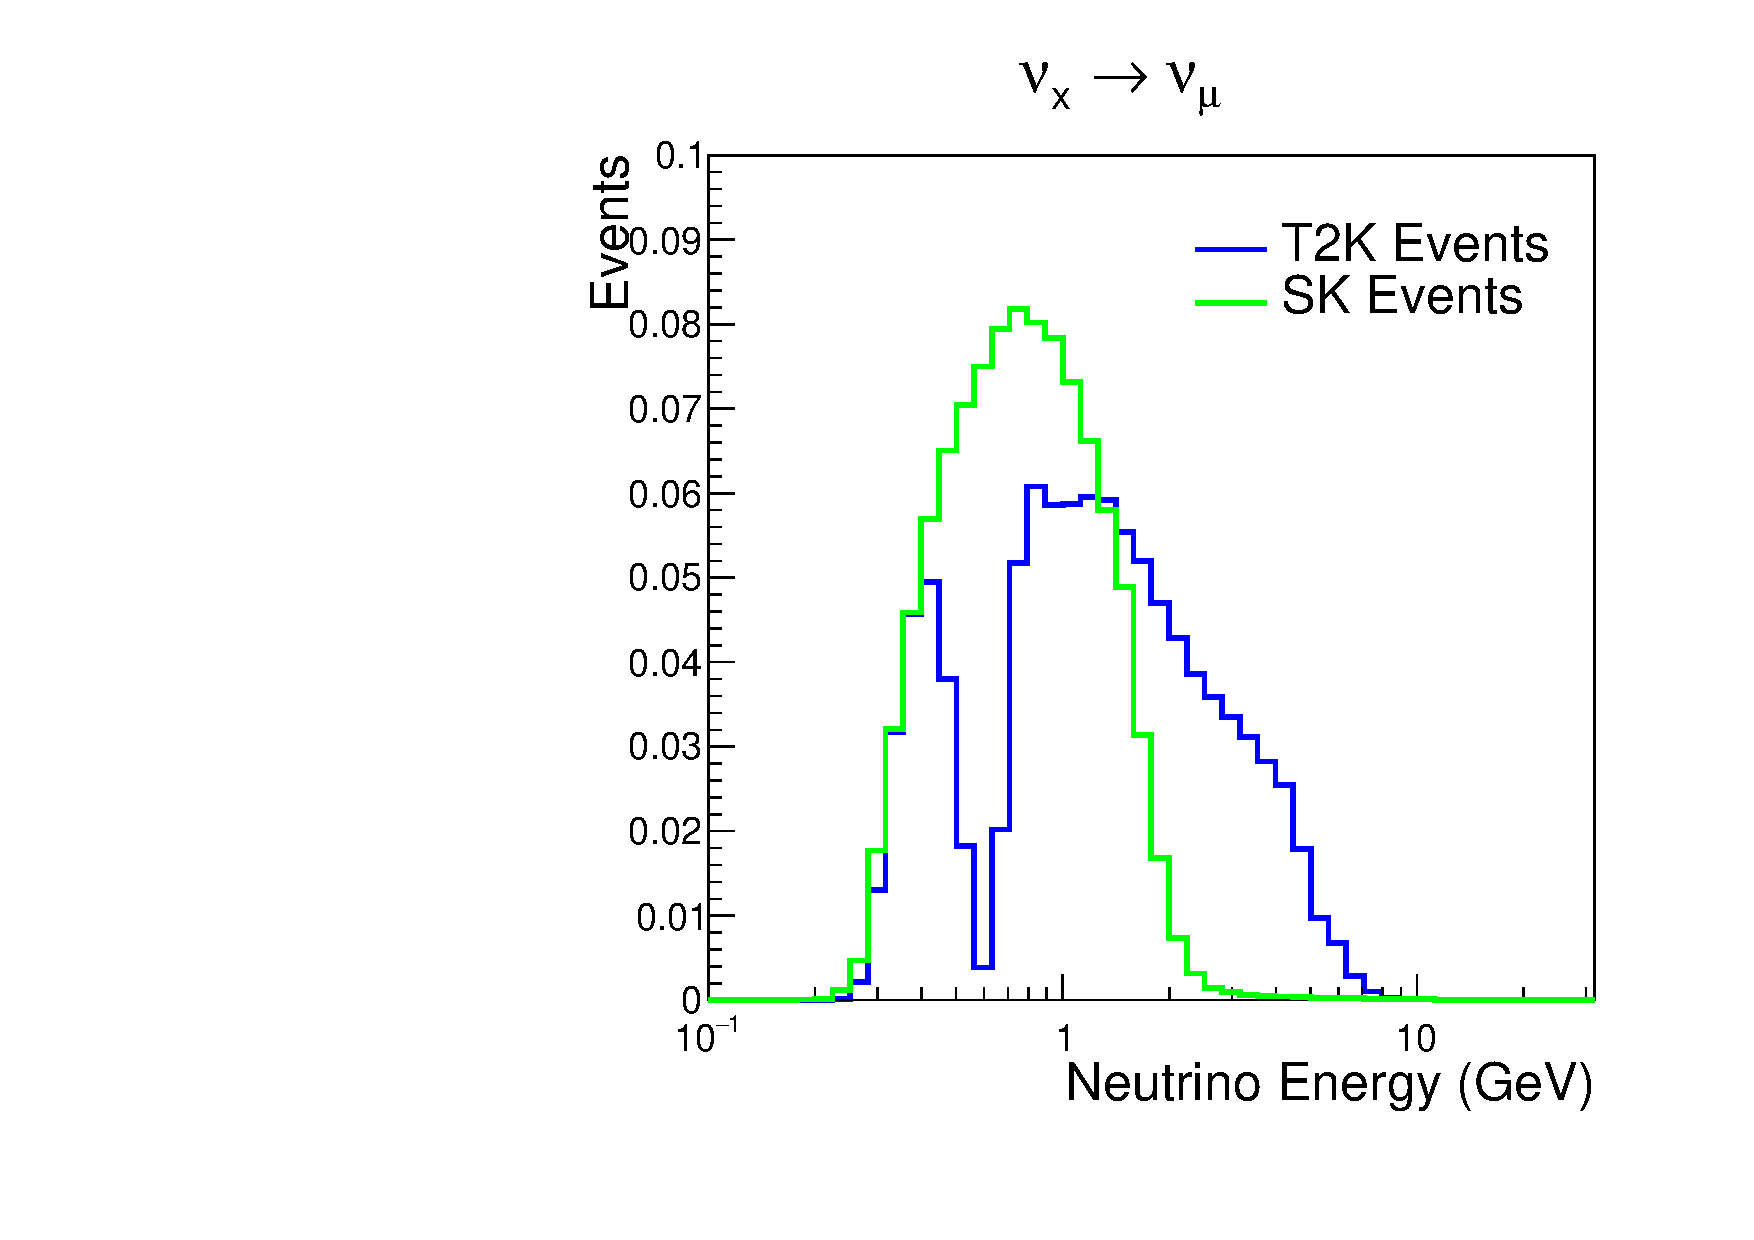
\includegraphics[width=\textwidth, trim={0mm 0mm 0mm 0mm}, clip,page=1]{Figures/Selections/NeutrinoEnergyDist_Comp_1Rmu_NuMu.pdf}
    \subcaption{\quickmath{\mu}-like}
  \end{subfigure}%
  \begin{subfigure}[t]{0.49\textwidth}
    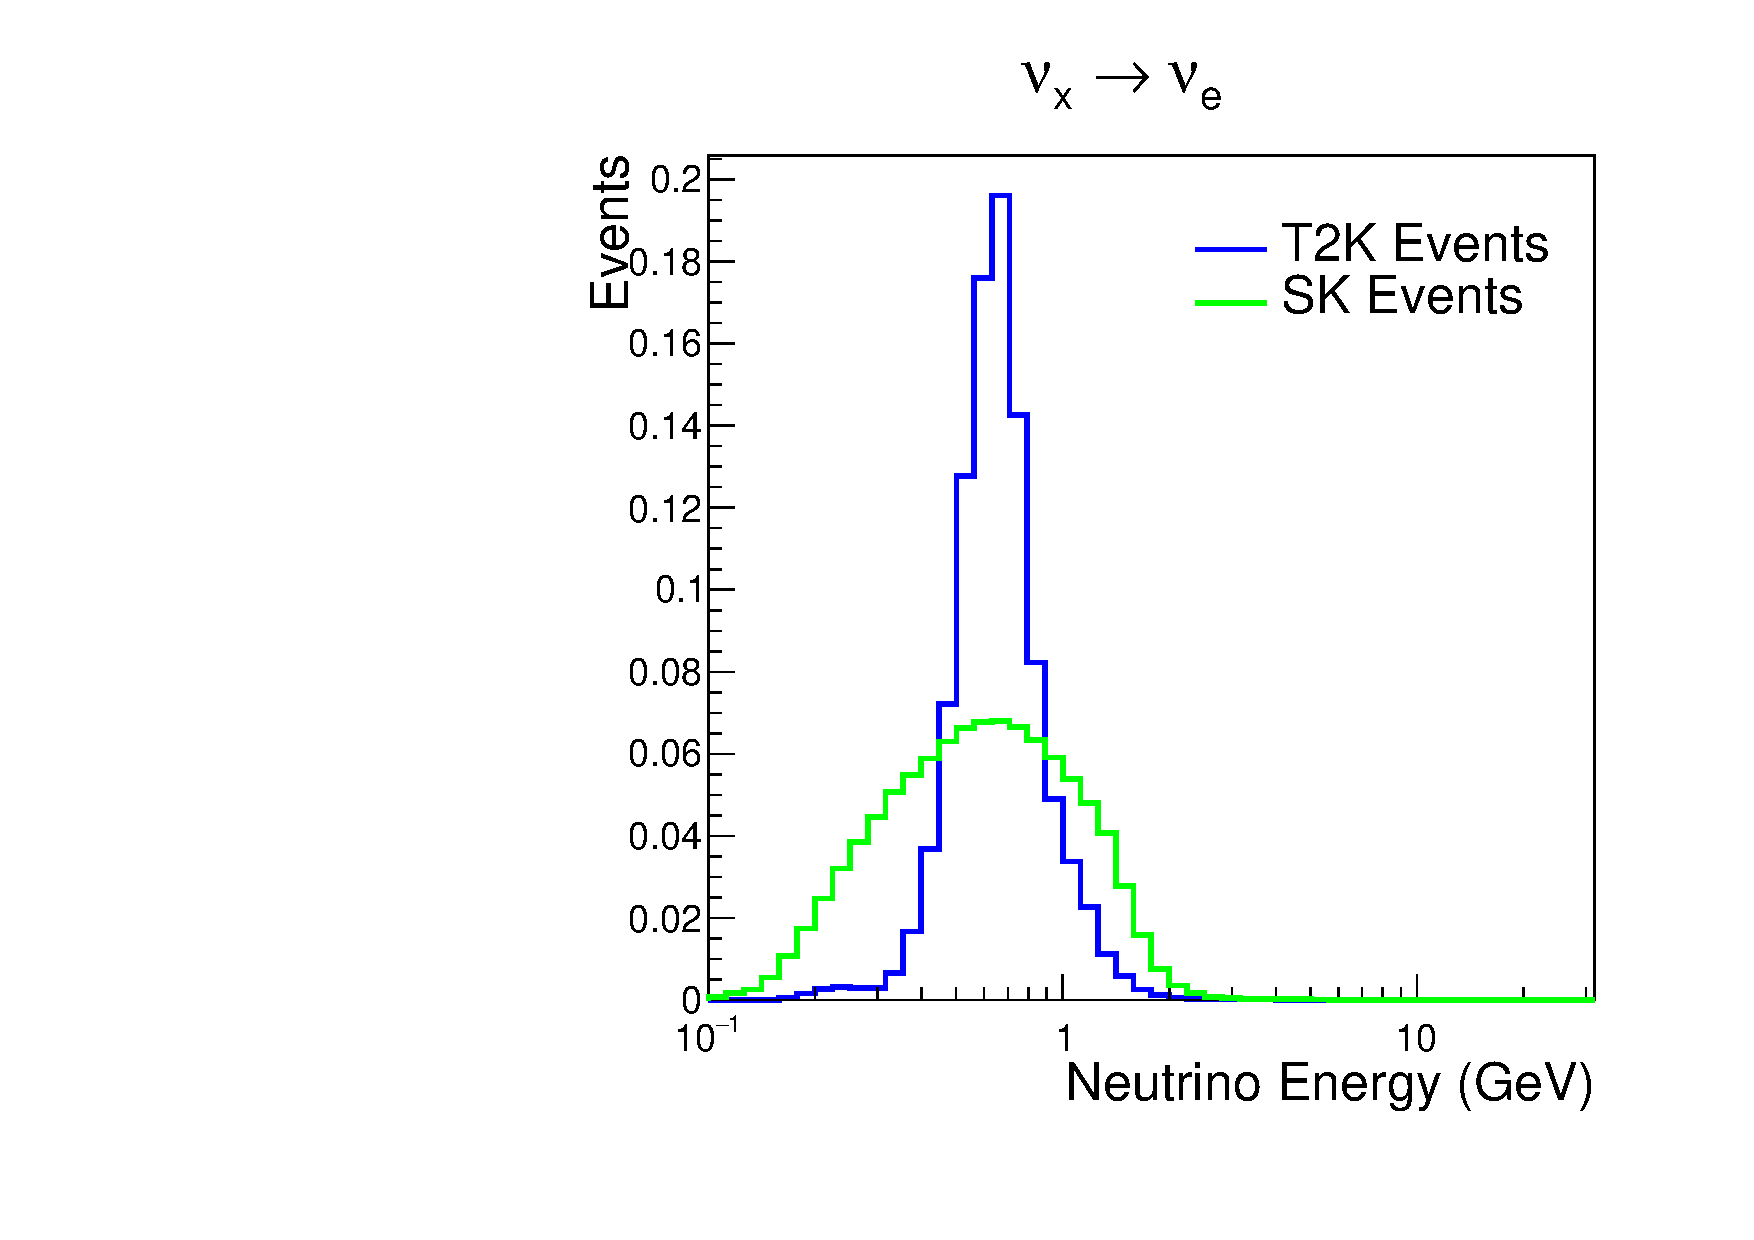
\includegraphics[width=\textwidth, trim={0mm 0mm 0mm 0mm}, clip,page=1]{Figures/Selections/NeutrinoEnergyDist_Comp_1Re_NuE.pdf}
    \subcaption{\quickmath{e}-like}
  \end{subfigure}
  \begin{subfigure}[t]{0.49\textwidth}
    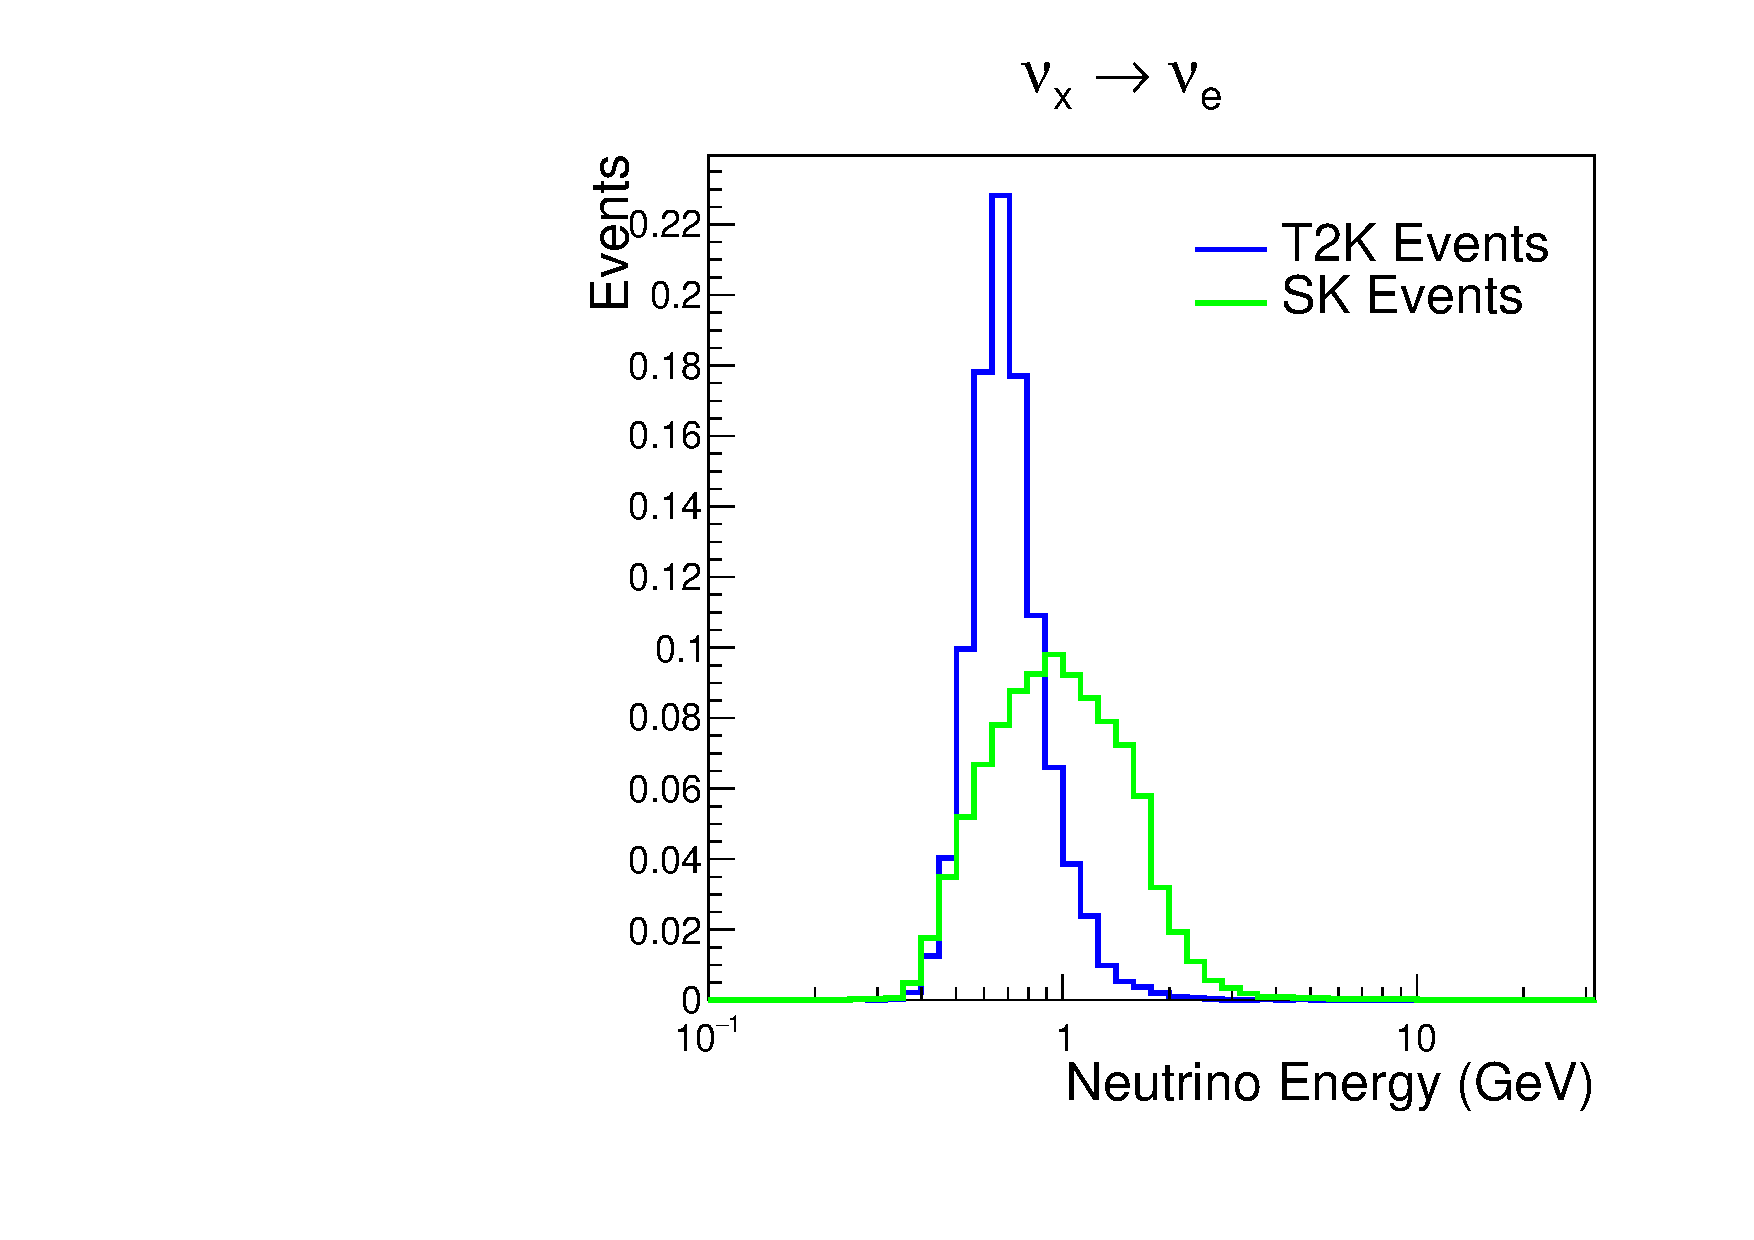
\includegraphics[width=\textwidth, trim={0mm 0mm 0mm 0mm}, clip,page=1]{Figures/Selections/NeutrinoEnergyDist_Comp_1Re1de_NuE.pdf}
    \subcaption{\quickmath{e}-like + 1d.e.}
  \end{subfigure}
  \caption{The prediction neutrino energy distribution for subGeV atmospheric and beam samples, given for muon-like samples FHC+RHC 1R\quickmath{\mu} beam samples compared to the subGeV \quickmath{\mu}-like 0+1 decay electrons (d.e.) atmospheric samples, electron-like 0d.e. samples FHC+RHC 1R\quickmath{e} beam samples compared to the subGeV \quickmath{e}-like 1d.e. sample, and electron-like 1d.e. sample FHC1Re1de beam sample compared to the subGeV \quickmath{e}-like 1d.e. atmospheric sample.}
  \label{fig:SelsAndSysts_NeutrinoEnergyComparison}
\end{figure}

\begin{figure}[h]
  \begin{subfigure}[t]{\textwidth}
    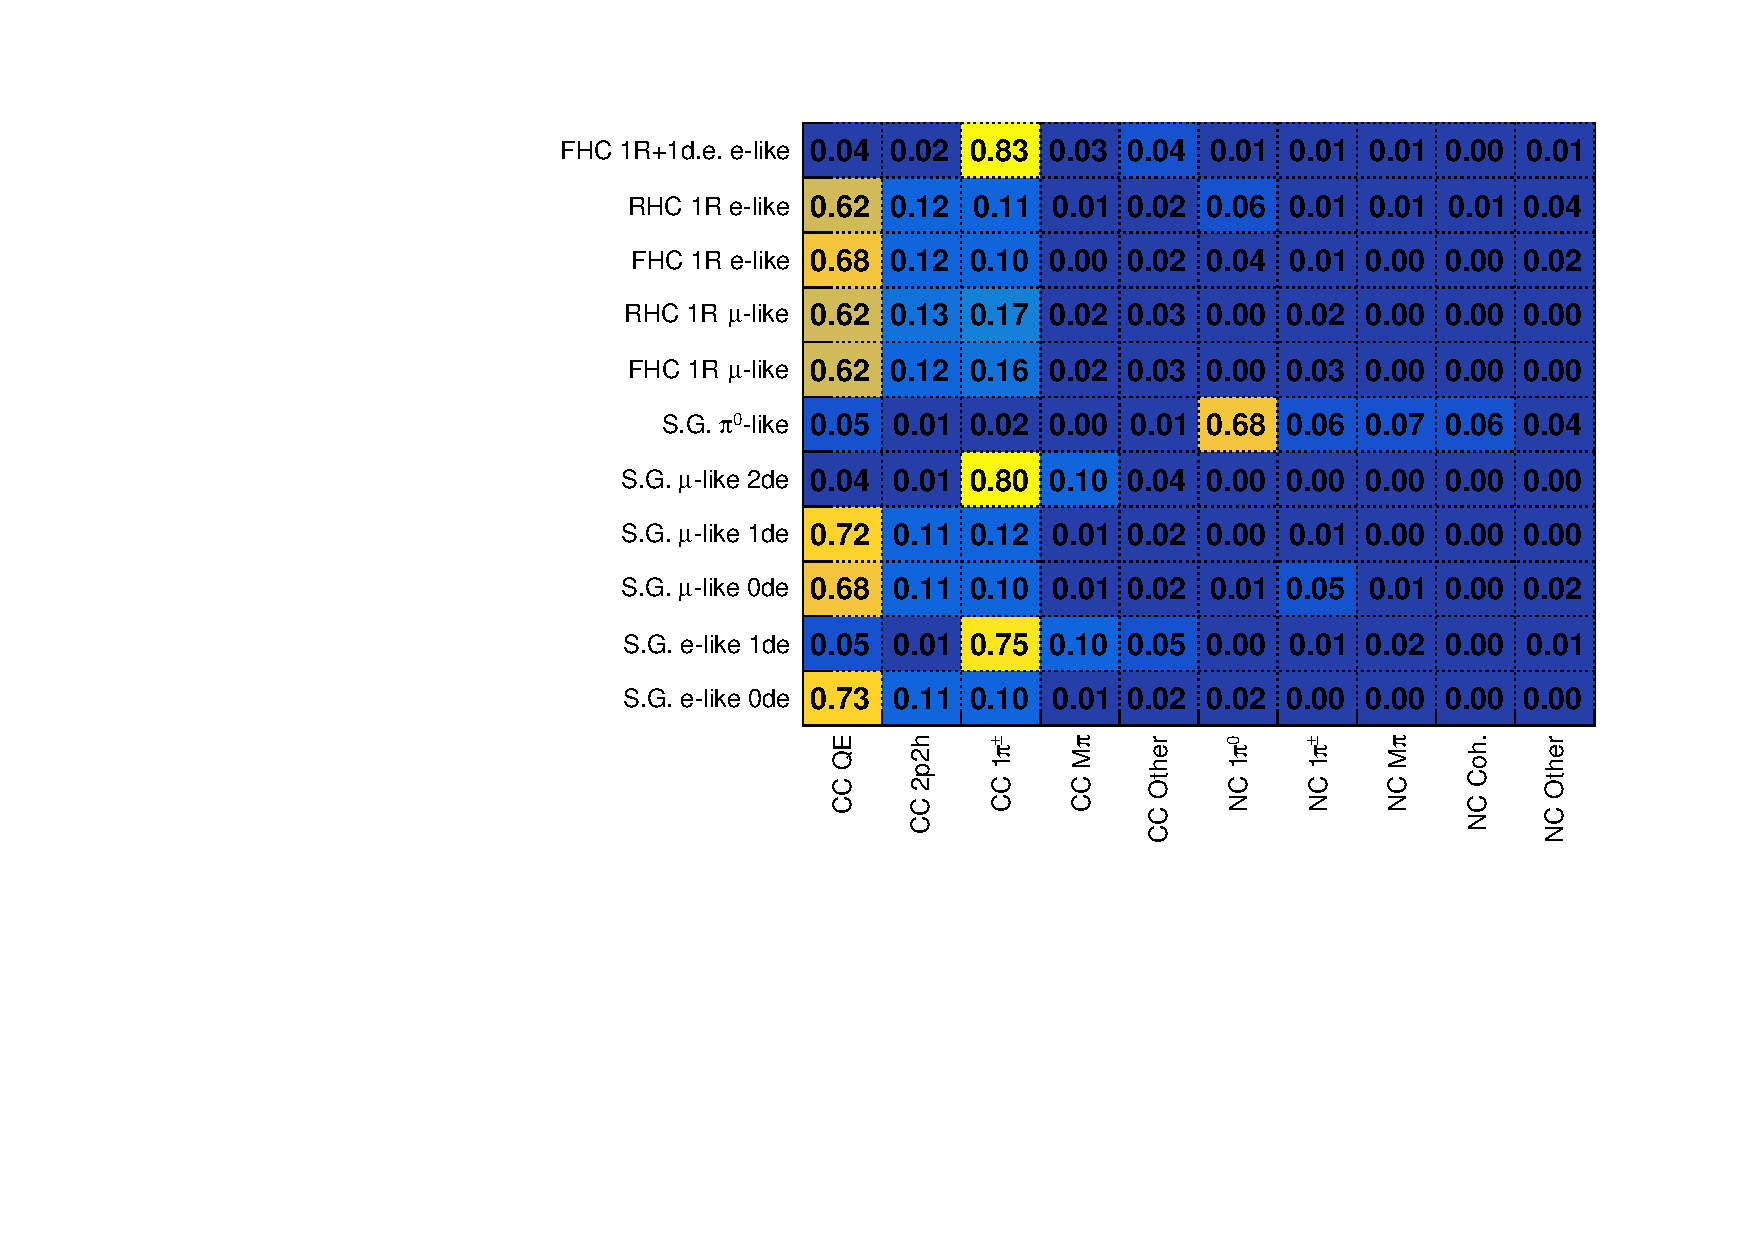
\includegraphics[width=\textwidth, trim={0mm 0mm 0mm 0mm}, clip,page=1]{Figures/Selections/FractionalModeComparison.pdf}
  \end{subfigure}
  \caption{The interaction mode contribution of each sample given as a fraction of the total event rate in that sample. All systematic dials are set to their nominal values and the Asimov A oscillation parameters are assumed. The Charged Current (CC) modes are broken into quasi-elastic (QE), meson exchange (2p2h), resonant charged pion production (\quickmath{1\pi^{\pm}}), multi-pion production (\quickmath{M\pi}), and other interaction category. Neutal Current (NC) interaction modes are given in interaction mode categories: \quickmath{\pi^{0}} production, resonant charged pion production,  multi-pion production and other.}
  \label{fig:SelsAndSysts_FractionalModeComparison}
\end{figure}

The T2K uncertainty model is applied in a similar methodology to the SK model parameters. It consists of \quickmath{19} shape parameters applied via third order polynominal splines and \quickmath{24} normalisation parameters. Four additional parameters, which model the uncertainty in the bining energy, are applied in a way to shift the momentum of lepton emitted from a nucleus. The majority of these parameters are assigned a Gaussian prior uncertainty. Those that have no theoretical reasoning, or those which have not been fit to external data, are assigned a flat prior which does not affect the penalty term. The CCQE model parameters were tuned to MiniBooNE \cite{miniboone_nu_ccqe} and MINER\quickmath{\nu}A \cite{minerva_nubar_ccqe} measurements and CCRES model parameters are tuned to ANL and BNL experiments \cite{ANL_BNL_corr}.

On top of the combination of the SK and T2K interaction models, several other parameters have been specifically developed for the joint oscillation analysis. As the majority of the atmospheric samples' \dcp sensitivity comes from the normalisation of subGeV electron-like events, additional dial which models an alternative Continous Random Phase Approximation (CRPA) nuclear ground state has been implemented \cite{t2k_tn_422}. As the near detector can not sufficiently constrain the model, this dial approximates the event weights if a CRPA model had been assumed rather than a spectral function. This dial only effects \quickmath{\nu_{e}} and \quickmath{\bar{\nu}_{e}} and is applied as a shape parameter.

Further additions to the model have been included due to the the subGeV \quickmath{\pi^{0}} atmospheric sample. This particulary targets charged current and neutral current \quickmath{\pi^{0}} producing interactions to constrain the systematic uncertainties. However, there is no analogous sample in the T2K beam-only analysis so no significant effort has been placed into building a sufficient uncertainty model. Therefore, an uncertainty which effects neutral current resonant \quickmath{\pi^{0}} production is incorporated in this analysis. Comparisons of NEUT's NC resonant pion production predictions have been made to MiniBooNE \cite{MB_NC1pi0} data and a consistent \quickmath{16\%} to \quickmath{21\%} underprediction is observed. Consequently, a conservative \quickmath{30\%} normalisation is invoked. 



